\section{伪随机函数:基本定义与性质}

虽然安全的分组密码是许多密码系统的组成部分,但一个与之密切相关的概念,即伪随机函数(PRF),被证明是许多应用中的正确工具。PRF在概念上比分组密码更加简单,正如我们将看到的,它们有着广泛的应用。PRF和分组密码密切相关,在某些假设下,我们可以用安全的分组密码作为安全伪随机函数的替身。这种性质非常有益,因为正如我们在上一节所看到的,我们已经有了许多非常实用的、貌似安全的分组密码。

\subsection{定义}

\textbf{伪随机函数 (Pseudo-random function, PRF)} $F$ 是一种确定性算法,它有两个输入:一个密钥 $k\in\mathcal{K}$ 和一个\textbf{输入数据分组} $x\in\mathcal{X}$;它的输出 $y:=F(k,x)\in\mathcal{Y}$ 被称为\textbf{输出数据分组}。我们称 $F$ \textbf{定义在} $(\mathcal{K},\mathcal{X},\mathcal{Y})$ \textbf{上}。

直观地讲,我们对伪随机函数的安全概念表明,对于一个随机选择的密钥 $k$,函数 $F(k,\cdot)$ 对于所有实际目的都应该是一个``看起来像"随机分布的一个从 $\mathcal{X}$ 到 $\mathcal{Y}$ 的映射。为了使这一概念更加精确,我们首先引入一些符号:
\[
{\rm Funs}[\mathcal{X},\mathcal{Y}]
\]
表示\emph{所有}函数 $f:\mathcal{X}\to\mathcal{Y}$ 构成的集合。这是一个非常大的集合,事实上:
\[
|{\rm Funs}[\mathcal{X},\mathcal{Y}]|=|\mathcal{Y}|^{|\mathcal{X}|}
\]

我们可以定义如下的攻击游戏:

\begin{game}[伪随机函数]\label{game:4-2}
对于一个给定的定义在 $(\mathcal{K},\mathcal{X},\mathcal{Y})$ 上的 PRF $F$,对于一个给定对手 $\mathcal{A}$,我们定义两个实验:实验$0$和实验$1$。对于$b=0,1$,我们定义:\\
\noindent\textbf{实验$b$:}
\begin{itemize}
	\item 挑战者按照如下方式选定 $f\in{\rm Funs}[\mathcal{X},\mathcal{Y}]$:
	\vspace{1pt}
	
	\hspace*{5pt} 如果 $b=0$:选取 $k\overset{\rm R}\leftarrow\mathcal{K}$,令 $f\leftarrow F(k,\cdot)$;\\
	\hspace*{5pt} 如果 $b=1$:选取 $f\overset{\rm R}\leftarrow{\rm Funs}[\mathcal{X},\mathcal{Y}]$。
	\item 对手向挑战者提交一连串的查询。\\
	对于 $i=1,2,\dots$,第 $i$ 次查询是一个输入数据分组 $x_i\in\mathcal{X}$。\\
	挑战者计算 $y_i\leftarrow f(x_i)\in\mathcal{Y}$,并将 $y_i$ 交给对手。
	\item 对手计算并输出一个比特 $\hat{b}\in\{0,1\}$。
\end{itemize}
对于 $b=0,1$,令 $W_b$ 为 $\mathcal{A}$ 在实验 $b$ 中输出 $1$ 的事件。我们将 $\mathcal{A}$ 相对于 $F$ 的\textbf{优势}定义为:
\begin{equation}\label{eq:4-21}
{\rm PRF\mathsf{adv}}[\mathcal{A}, F]:=
\Big\lvert
{\rm Pr}[W_0]-{\rm Pr}[W_1]
\Big\rvert
\end{equation}
如果对手 $\mathcal{A}$ 最多发出 $Q$ 次查询,我们就称 $\mathcal{A}$ 是一个 \textbf{$Q$ 次查询伪随机函数对手($Q$-query PRF adversary)}。
\end{game}

\begin{definition}[安全的 PRF]\label{def:4-2}
如果对于所有的有效对手 $\mathcal{A}$,${\rm PRF\mathsf{adv}}[\mathcal{A},F]$ 的值都可忽略不计,我们就称伪随机函数 $F$ 是\textbf{安全的}。
\end{definition}

需要再次强调,在攻击游戏 \ref{game:4-2} 中,对手所做的查询可以是自适应的:对手可以根据挑战者之前应答的内容来构造每个新的查询(见练习 4.6)。

正如 \ref{subsec:2-2-5} 小节所讨论的,攻击游戏 \ref{game:4-2} 可以被重构为一个``比特猜测"游戏。在该游戏中,挑战者并不运行两个独立的实验,而是随机选择一个 $b\in\{0,1\}$,然后针对对手 $\mathcal{A}$ 运行实验 $b$。在这个游戏中,我们令 $\mathcal{A}$ 的比特猜测优势 ${\rm PRF\mathsf{adv}}^*[\mathcal{A}, F]$ 为 $|{\rm Pr}[\hat{b}=b]-{1}/{2}|$。那么,\ref{subsec:2-2-5} 小节中的推广结论(即式 \ref{eq:2-11})在此也适用:
\begin{equation}
{\rm PRF\mathsf{adv}}[\mathcal{A}, F]=2\cdot {\rm PRF\mathsf{adv}}^*[\mathcal{A}, F]
\end{equation}

\begin{snote}[弱安全的伪随机函数。]
对于某些使用 PRF 的构造来说,PRF 满足比定义 \ref{def:4-2} 更弱的安全属性也就足够了。我们说,如果对手的查询受到严格限制,但仍没有有效对手能够将 PRF 与随机函数区分开来时,我们就说该 PRF 是\emph{弱安全的}。所谓的查询的严格限制,指的是对手只能在域中的\emph{随机}点上查询函数。将对手的查询限制在随机输入上,就有可能更容易建立弱安全的 PRF。在练习 4.2 中,我们会研究弱安全但不完全安全的自然 PRF 构造。

我们通过稍微修改攻击游戏 \ref{game:4-2} 来定义弱安全的 PRF。假设 $F$ 是一个定义在 $(\mathcal{K},\mathcal{X},\mathcal{Y})$ 上的 PRF。现在,我们修改对手 $\mathcal{A}$ 与挑战者的交互方式:每当对手 $\mathcal{A}$ 查询函数时,挑战者都选择一个随机数 $x\in\mathcal{X}$,并将 $x$ 与 $f(x)$ 都发送给对手。换句话说,对手 $\mathcal{A}$ 看到的是函数 $f$ 在 $\mathcal{X}$ 上的一个\emph{随机}点上的评估结果,并且需要判断该函数是真正的随机函数还是一个伪随机函数。我们将对手 $\mathcal{A}$ 在该游戏中的优势定义为 ${\rm wPRF\mathsf{adv}}[\mathcal{A}, F]$,如式 \ref{eq:4-21} 所示。
\end{snote}

\begin{definition}[弱安全的 PRF]\label{def:4-3}
如果对于所有的有效对手 $\mathcal{A}$, ${\rm wPRF\mathsf{adv}}[\mathcal{A}, F]$ 的值都可忽略不计,我们就称伪随机函数 $F$ 是\textbf{弱安全的}。
\end{definition}

\subsection{随机函数的有效实现}\label{subsec:4-4-2}

同 \ref{subsec:4-1-2} 小节一样,我们可以通过一个\textbf{忠实的侏儒}来实现攻击游戏 \ref{game:4-2} 的实验 $1$ 中挑战者使用的从 ${\rm Funs}[\mathcal{X},\mathcal{Y}]$ 中选出的随机函数。同分组密码的情况一样,挑战者会跟踪输入/输出对 $(x_i,y_i)$。当挑战者收到第 $i$ 次查询 $x_i$ 时,他需要验证是否存在某个 $j < i$ 使得 $x_i=x_j$ 成立。如果存在,他就令 $y_i\leftarrow y_j$(这确保挑战者确实实现了一个函数),否则就从集合 $\mathcal{Y}$ 中随机选择一个 $y_i$;最后,挑战者将 $y_i$ 发送给对手。我们可以把挑战者的这种实现逻辑表述如下:

\vspace{5pt}

\hspace*{5pt} 当从对手 $\mathcal{A}$ 处收到第 $i$ 个查询 $x_i\in\mathcal{X}$ 时:\\
\hspace*{50pt} 如果存在某个 $j<i$ 使得 $x_i=x_j$ 成立:\\
\hspace*{75pt} 令 $y_i\leftarrow y_j$\\
\hspace*{75pt} 否则,选取 $y_i\overset{\rm R}\leftarrow\mathcal{Y}$\\
\hspace*{50pt} 将 $y_i$ 发送给 $\mathcal{A}$。\\

\subsection{什么时候一个安全的分组密码是安全的PRF?}

在本小节的开始,我们提出一个问题:什么时候一个安全分组密码才是一个安全的 PRF?在回答这个问题时,我们要介绍一种在整个密码学中被大量使用的证明技术。

令 $\mathcal{E}=(E,D)$ 是一个定义在 $(\mathcal{K},\mathcal{X})$ 上的分组密码,并令 $N:=|\mathcal{X}|$。我们可以自然地把 $\mathcal{E}$ 看作是一个定义在 $(\mathcal{K},\mathcal{X},\mathcal{X})$ 上的 PRF。现在假设 $\mathcal{E}$ 是一个安全分组密码,也就是说,不存在有效对手能够有效地将 $\mathcal{E}$ 与随机置换区分开来。这是否意味着 $\mathcal{E}$ 也是一个安全的 PRF 呢?也即,这是否意味着不存在有效对手可以有效地将 $\mathcal{E}$ 与随机函数区分开来?

这个问题的答案是``是",前提是 $N$ 是超多项式的。在论证这个问题之前,我们需要先论证,当 $N$ 很小的时候,上述问题的答案``否"。

考虑一个 PRF 对手,它对 $\mathcal{E}$ 进行攻击游戏 \ref{game:4-2} 中所描述的攻击,令 $f$ 是挑战者选择的函数:在实验 $0$ 中,$f=E(k,\cdot)$,其中 $k\in\mathcal{K}$ 为一随机值;而在实验 $1$ 中,$f$ 是从 ${\rm Funs}[\mathcal{X},\mathcal{Y}]$ 中随机选出的。假设 $N$ 是如此之小,以至于一个有效对手可以对所有的 $x\in\mathcal{X}$ 计算 $f(x)$ 的值。此外,如果对手 $\mathcal{A}$ 看到了两个不同的 $x,x'\in\mathcal{X}$ 使得 $f(x)=f(x')$,它就输出 $1$,否则就输出 $0$。显然,在实验 $0$ 中,$\mathcal{A}$ 输出 $1$ 的概率为 $0$,因为此时 $f=E(k,\cdot)$ 是一个置换。然而,在实验 $1$ 中,$\mathcal{A}$ 能以 $1-{N!}/{N^N}\geq{1}/{2}$ 的概率输出 $1$。因此我们有 ${\rm PRF\mathsf{adv}}[\mathcal{A}, F]\geq\frac{1}{2}$,所以 $\mathcal{E}$ 不是一个安全的 PRF。

上述论证可以用生日悖论来完善(见 \ref{sec:B-1} 节)。对于任何多项式边界的 $Q$,我们可以定义一个有效 PRF 对手 $\mathcal{A}$,它对 $\mathcal{E}$ 进行攻击游戏 \ref{game:4-2} 中的攻击,流程如下所述。对手 $\mathcal{A}$ 只需向挑战者发出 $Q$ 个不同的查询,当且仅当它能得到两个不同的值 $x,x'\in\mathcal{X}$ (从给挑战者的$Q$个值中选出)使得 $f(x)=f(x')$时,输出 $1$。同样,在实验 $0$ 中,$\mathcal{A}$ 输出 $1$ 的概率为 $0$。然而,根据定理 \ref{theo:B-1},在实验 $1$ 中,$\mathcal{A}$ 输出 $1$ 的概率至少为 $\min\{{Q(Q-1)}/{4N},0.63\}$。因此,只需进行 $O(N^{1/2})$ 次查询,对手就可以很容易地看到,置换的行为并不像是一个随机函数。

事实证明,``生日攻击"是所有对手所能达到的最好情况。当 $N$ 是超多项式的时候,这种攻击就变得不再可行了。

\begin{theorem}[PRF 切换引理]\label{theo:4-4}
令 $\mathcal{E}=(E,D)$ 是一个定义在 $(\mathcal{K},\mathcal{X})$ 上的分组密码,并令 $N:=|\mathcal{X}|$。令 $\mathcal{A}$ 是一个对手,它最多向挑战者发起 $Q$ 次查询。则有:
\[
\Big\lvert
{\rm BC\mathsf{adv}}[\mathcal{A},\mathcal{E}]-{\rm PRF\mathsf{adv}}[\mathcal{A},\mathcal{E}]
\Big\rvert
\leq{Q^2}/{2N}
\]
\end{theorem}

在证明这个定理之前,我们先导出下面的一个简单的推论。

\begin{corollary}\label{cor:4-5}
令 $\mathcal{E}=(E,D)$ 是一个定义在 $(\mathcal{K},\mathcal{X})$ 上的分组密码,并假设 $N:=|\mathcal{X}|$ 是超多项式的。那么,当且仅当 $\mathcal{E}$ 是一个安全的 PRF 时,$\mathcal{E}$ 是一个安全的分组密码。
\end{corollary}

\begin{proof}
根据定义,如果 $\mathcal{A}$ 是一个有效对手,它向挑战者发出的最大查询次数 $Q$ 是多项式边界的。因此,根据定理 \ref{theo:4-4},我们有:
\[
\Big\lvert
{\rm BC\mathsf{adv}}[\mathcal{A},\mathcal{E}]-{\rm PRF\mathsf{adv}}[\mathcal{A},\mathcal{E}]
\Big\rvert
\leq{Q^2}/{2N}
\]
由于 $N$ 是超多项式的,$Q$ 是多项式边界的,所以 $\frac{Q^2}{2N}$ 是可以忽略不计的(见事实 \ref{fact:2-6})。由此可见,当且仅当 ${\rm PRF\mathsf{adv}}[\mathcal{A},\mathcal{E}]$ 可忽略不计时,${\rm BC\mathsf{adv}}[\mathcal{A},\mathcal{E}]$ 才是可以忽略不计的。
\end{proof}

实际上,定理 \ref{theo:4-4} 的证明与分组密码和 PRF 无关,它实际上是一个关于随机置换和随机函数的论证。让我们定义一个新的攻击游戏,用以测试对手区分随机置换与随机函数的能力。

\begin{game}[置换 \emph{vs.} 函数]\label{game:4-3}
对于一个给定有限集 $\mathcal{X}$ 和一个给定对手 $\mathcal{A}$,我们定义两个实验:实验$0$和实验$1$。对于$b=0,1$,我们定义:\\
\textbf{实验$b$:}
\begin{itemize}
	\item 挑战者按照如下方式选定 $f\in{\rm Funs}[\mathcal{X},\mathcal{X}]$:
	\vspace{1pt}
	
	\hspace*{5pt} 如果 $b=0$:选取 $f\overset{\rm R}\leftarrow{\rm Perms}[\mathcal{X}]$;\\
	\hspace*{5pt} 如果 $b=1$:选取 $f\overset{\rm R}\leftarrow{\rm Funs}[\mathcal{X},\mathcal{X}]$。
	\item 对手向挑战者提交一连串的查询。\\
	对于 $i=1,2,\dots$,第 $i$ 次查询是一个输入数据分组 $x_i\in\mathcal{X}$。\\
	挑战者计算 $y_i\leftarrow f(x_i)\in\mathcal{Y}$,并将 $y_i$ 交给对手。
	\item 对手计算并输出一个比特 $\hat{b}\in\{0,1\}$。
\end{itemize}
对于 $b=0,1$,令 $W_b$ 为 $\mathcal{A}$ 在实验 $b$ 中输出 $1$ 的事件。我们将 $\mathcal{A}$ 相对于 $\mathcal{X}$ 的\textbf{优势}定义为:
\[
{\rm PF\mathsf{adv}}[\mathcal{A}, \mathcal{X}]:=
\Big\lvert
{\rm Pr}[W_0]-{\rm Pr}[W_1]
\Big\rvert
\]
\end{game}

\begin{theorem}\label{theo:4-6}
令 $\mathcal{X}$ 是一个大小为 $N$ 的有限集,$\mathcal{A}$ 是一个对手,它最多向挑战者发起 $Q$ 次查询,则有:
\[
{\rm PF\mathsf{adv}}[\mathcal{A},\mathcal{X}]\leq{Q^2}/{2N}
\]
\end{theorem}


我们首先表明,上面的定理很容易推出定理 \ref{theo:4-4}。

\begin{proof}[定理 \ref{theo:4-4} 的证明]
令 $\mathcal{E}=(E,D)$ 是一个定义在 $(\mathcal{K},\mathcal{X})$ 上的分组密码。令 $\mathcal{A}$ 是一个对手,它最多向挑战者发起 $Q$ 次查询。我们定义游戏 $0$、游戏 $1$ 和游戏 $2$,它们都在 $\mathcal{A}$ 和挑战者之间进行。对于 $j=0,1,2$,我们定义 $p_j$ 为 $\mathcal{A}$ 在游戏 $j$ 中输出 $1$ 的概率。在每个游戏中,挑战者根据特定的分布选择一个函数 $f:\mathcal{X}\to\mathcal{X}$,并以 $f(x)$ 来应答 $\mathcal{A}$ 的每个查询 $x\in\mathcal{X}$。

\noindent\textbf{游戏 $\mathbf{0}$}:该游戏中的挑战者令 $f:=E(k,\cdot)$,其中 $k\in\mathcal{K}$ 是随机选出的。

\noindent\textbf{游戏 $\mathbf{1}$}:该游戏中的挑战者随机选择 $f\in{\rm Perms}[\mathcal{X}]$。

\noindent\textbf{游戏 $\mathbf{2}$}:该游戏中的挑战者随机选择 $f\in{\rm Funs}[\mathcal{X},\mathcal{X}]$。

注意到,根据定义,有:
\[
\begin{aligned}
	& |p_1-p_0| = {\rm BC\mathsf{adv}}[\mathcal{A},\mathcal{E}]\\
	& |p_2-p_0| = {\rm PRF\mathsf{adv}}[\mathcal{A},\mathcal{E}]
\end{aligned}
\]
而根据定理 \ref{theo:4-6},有:
\[
|p_2-p_1|={\rm PF\mathsf{adv}}[\mathcal{A},\mathcal{X}]\leq{Q^2}/{2N}
\]
将上两式结合,我们得到:
\[
\big\lvert
{\rm BC\mathsf{adv}}[\mathcal{A},\mathcal{E}]-{\rm PRF\mathsf{adv}}[\mathcal{A},\mathcal{E}]
\big\rvert
=
\big\lvert
|p_1-p_0|-|p_2-p_0|
\big\rvert
\leq|p_2-p_1|\leq{Q^2}/{2N}
\]

这就证明了该定理。
\end{proof}

所以,剩下工作的就是证明定理 \ref{theo:4-6}。在此之前,我们要说明一个非常简单但非常有用的结论:

\begin{theorem}[差分引理]\label{theo:4-7}
令 $Z$,$W_0$,$W_1$ 是定义在某个概率空间上的事件。假设当且仅当 $W_1\land\bar Z$ 发生时,$W_0\land\bar Z$ 才发生,则我们有:
\[
|\Pr[W_0]-\Pr[W_1]|\leq\Pr[Z]
\]
\end{theorem}

\begin{proof}
这就是一个简单的计算。我们有:
\[
\begin{aligned}
|\Pr[W_0]-\Pr[W_1]|
&=|\Pr[W_0\land Z]+\Pr[W_0\land\bar Z]-\Pr[W_1\land Z]-\Pr[W_1\land\bar Z]|\\
&=|\Pr[W_0\land Z]-\Pr[W_1\land Z]|\\
&\leq \Pr[Z]
\end{aligned}
\]
其中第二个等式来自 $W_0\land\bar{Z} \Longleftrightarrow W_1\land\bar{Z}$ 的假设,所以,一个特殊结论就是 $\Pr[W_0\land\bar{Z}]=\Pr[W_1\land\bar{Z}]$。最后的不等式来自于这样一个事实,即 $\Pr[W_0\land Z]$ 和 $\Pr[W_1\land Z]$ 都是介于 $0$ 和 $\Pr[Z]$ 之间的值。
\end{proof}
 
在我们对差分定理的大多数应用中,$W_0$ 代表一个给定对手在对某个挑战者的游戏中输出 $1$ 的事件,而 $W_1$ 则是同一个对手在对另一个挑战者的游戏中输出 $1$ 的事件。为了应用差分定理,我们定义这两个游戏,使它们都在相同的基础概率空间上运行。这意味着我们假设对手和挑战者在两个游戏中所做的随机选择都是一样的,两个游戏的不同之处仅在于挑战者针对来自对手的查询给出反馈的策略。

\begin{proof}[定理 \ref{theo:4-6} 的证明]
考虑一个对手 $\mathcal{A}$,它对 $\mathcal{X}$ 进行攻击游戏 \ref{game:4-3} 中的攻击,其中 $N:=|\mathcal{X}|$,并假设 $\mathcal{A}$ 最多向挑战者发起 $Q$ 次查询。考虑这个攻击游戏的实验 $0$。利用 \ref{subsec:4-4-2} 小节讨论的``忠实的侏儒"的思想,我们可以通过跟踪输入/输出对 $(x_i,y_i)$ 来实现实验 $0$;此外,为 $y_i$ 选择初始的``默认"值 $z_i$ 是很方便的,$z_1,\dots,z_Q$ 可以从 $\mathcal{X}$ 中均匀独立随机选出;这些``默认"值在必要时可以被覆写,以确保挑战者定义的是一个随机置换。下面是详细的过程:

\vspace{5pt}

\hspace*{5pt} 选取 $z_1,\dots,z_Q\overset{\rm R}\leftarrow\mathcal{X}$\\
\hspace*{26pt} 当收到 $\mathcal{A}$ 的第 $i$ 个查询 $x_i$ 时:\\
\hspace*{50pt} 如果存在某个 $j<i$ 使得 $x_i=x_j$,则:\\
\hspace*{75pt} 令 $y_i\leftarrow y_j$\\
\hspace*{50pt} 否则:\\
\hspace*{75pt} 令 $y_i\leftarrow z_i$\\
\hspace*{1pt} ($*$)
\hspace*{53pt} 如果 $y_i\in\{y_1,\dots,y_{i-1}\}$,则选取 $y_i\overset{\rm R}\leftarrow\mathcal{X}\setminus\{y_1,\dots,y_{i-1}\}$;\\
\hspace*{50pt} 将 $y_i$ 发送给 $\mathcal{A}$。

\vspace{5pt}

标有 ($*$) 的那行用于测试是否需要覆盖默认值 $z_i$,确保没有任何输出值被用于两个不同的输入值。

令 $W_0$ 为 $\mathcal{A}$ 在该游戏中输出 $1$ 的事件,我们称之为游戏 $0$。

我们现在修改上述挑战者的实现,得到另一个新的游戏:

\vspace{5pt}

\hspace*{5pt} 选取 $z_1,\dots,z_Q\overset{\rm R}\leftarrow\mathcal{X}$\\
\hspace*{26pt} 当收到 $\mathcal{A}$ 的第 $i$ 个查询 $x_i$ 时:\\
\hspace*{50pt} 如果存在某个 $j<i$ 使得 $x_i=x_j$,则:\\
\hspace*{75pt} 令 $y_i\leftarrow y_j$\\
\hspace*{50pt} 否则:\\
\hspace*{75pt} 令 $y_i\leftarrow z_i$\\
\hspace*{50pt} 将 $y_i$ 发送给 $\mathcal{A}$。

\vspace{5pt}

我们所做的只是在原来的挑战者逻辑中删除了标有 ($*$) 的那行,这使得我们``忠实的侏儒"变成了一个``健忘的侏儒",他忘记了检查输出值是否存在重复。

令 $W_1$ 为 $\mathcal{A}$ 在与这个修改后的挑战者进行的游戏中输出 $1$ 的事件,我们称之为游戏 $1$。

请注意,游戏 $1$ 等同于攻击游戏 \ref{game:4-3} 的实验 $1$;特别地,$\Pr[W_1]$ 等于 $\mathcal{A}$ 在攻击游戏 \ref{game:4-3} 的实验 $1$ 中输出 $1$ 的概率。因此,我们有:
\[
{\rm PF\mathsf{adv}}[\mathcal{A},\mathcal{X}]=|\Pr[W_0]-\Pr[W_1]|
\]

我们现在应用差分引理。为此,上述两个游戏都被假设运行在相同的基础概率空间上。在这两个游戏中,对手和挑战者所做的所有随机选择都是一样的,唯一不同的是挑战者用来给出应答的规则。特别地,这意味着 $\mathcal{A}$ 的随机选择和挑战者选择的值 $z_1,\dots,z_Q$ 不仅具有相同的分布,而且在两个游戏中都是\emph{确确实实的相同值}。

定义 $Z$ 为存在某个 $i\neq j$ 使得 $z_i=z_j$ 成立的事件。现在,假设我们运行游戏 $0$ 和游戏 $1$,而事件 $Z$ 没有发生。这意味着 $z_i$ 的值都是不同的。现在,由于对手的随机选择在两个游戏中都是相同的,它在两个游戏中的第一次查询也是相同的,因此挑战者的应答在两个游戏中也是相同的。对手的第二次查询(是其随机选择和挑战者第一次应答的函数)在两个游戏中也都是一样的。由于我们假设 $Z$ 没有发生,挑战者的应答在两个游戏中是相同的。继续这个论证,我们可以看到,对手的每次查询和挑战者的每个应答在两个游戏中都是一样的,因此对手的输出在两个游戏中都是一样的。因此,如果 $Z$ 没有发生,对手在游戏 $0$ 中输出 $1$,那么它在游戏 $1$ 中也会输出 $1$。同样地,如果 $Z$ 没有发生,而对手在游戏 $1$ 中输出 $1$,那么他在游戏 $0$ 中也会输出 $1$。更简洁地说,当且仅当 $W_1\land\bar{Z}$ 发生时,我们有 $W_0\land\bar{Z}$ 发生。因此,差分引理适用于该场景,我们得到:
\[
|\Pr[W_0]-\Pr[W_1]|\leq\Pr[Z]
\]

剩下的就是确定 $\Pr[Z]$ 的上界。这可由联合约束得到:对于任意不同索引对 $(i,j)$,必有$\Pr[z_i=z_j]={1}/{N}$,由于这样的索引对至多有 ${Q^2}/{2}$ 对,因此有:
\[
\Pr[Z]\leq{Q^2}/{2N}
\]
因此该定理得证。
\end{proof}

尽管还有其他的策略可以用来证明前面的定理(见练习 4.24),但我们在上面的证明中所使用的\textbf{健忘的侏儒}技术是非常有用的,我们将在后面的文章中多次看到它。

\subsection{使用 PRF 构建 PRG}\label{subsec:4-4-4}

由一个 PRF 构造一个 PRG 是很容易的。令 $F$ 是一个定义在 $(\mathcal{K},\mathcal{X},\mathcal{Y})$ 上的 PRF,$l\geq1$ 是一个多项式边界的值,令 $x_1,\dots,x_l$ 是 $\mathcal{X}$ 中任意固定且互不相同的元素(这要求$|\mathcal{X}|\geq l$)。我们定义一个具有种子空间 $\mathcal{K}$ 和输出空间 $\mathcal{Y}^l$ 的 PRG 如下:对于 $k\in\mathcal{K}$:
\[
G(k):=
\big(
F(k,x_1),\dots,F(k,x_l)
\big)
\]

\begin{theorem}\label{theo:4-8}
如果 $F$ 是一个安全的 PRF,那么上述 PRG $G$ 就是一个安全的 PRG。
\begin{quote}
特别地,对于每一个就 $G$ 进行攻击游戏 \ref{game:3-1} 的 PRG 对手 $\mathcal{A}$,都存在一个就 $F$ 进行攻击游戏 \ref{game:4-2} 的 PRF 对手 $\mathcal{B}$,其中 $\mathcal{B}$ 是围绕 $\mathcal{A}$ 的一个基本包装器,满足:
\end{quote}
\[
\mathrm{PRG}\mathsf{adv}[\mathcal{A},G]= 
\mathrm{PRF}\mathsf{adv}[\mathcal{B},F]
\]
\end{theorem}

\begin{proof}
令 $\mathcal{A}$ 是一个有效 PRG 对手,他对 G 进行攻击游戏 \ref{game:3-1} 中的攻击。我们描述一个相应的 PRF 对手 $\mathcal{B}$,他对 $F$ 进行攻击游戏 \ref{game:4-2} 中的攻击。对手 $\mathcal{B}$ 的工作方式如下:
\begin{quote}
$\mathcal{B}$ 向他的挑战者发起查询 $x_1,\dots,x_\ell$ 并获得应答 $y_1,\dots,y_\ell$。然后,对手 $\mathcal{B}$ 扮演 $\mathcal{A}$ 的挑战者的角色,向 $\mathcal{A}$ 发送 $(y_1,\dots,y_\ell)$。最后,对手 $\mathcal{B}$ 原样输出 $\mathcal{A}$ 所输出的所有东西。
\end{quote}

从构造上看,对于 $b=0,1$,$\mathcal{B}$ 在攻击游戏 \ref{game:4-2} 的实验 $b$ 相对于 $F$ 输出 $1$ 的概率恰好等于 $\mathcal{A}$ 在攻击游戏 \ref{game:3-1} 的实验 $b$ 相对于 $G$ 输出 $1$ 的概率,因此定理立即得证。
\end{proof}

\subsubsection{确定性计数器模式}

上述构造为我们提供了另一种从安全分组密码中建立语义安全密码的方法。假设 $\mathcal{E}=(E,D)$ 是一个定义在 $(\mathcal{K},\mathcal{X})$ 上的分组密码,其中 $\mathcal{X}=\{0,1\}^n$。令 $N:=|\mathcal{X}|=2^n$,假设 $N$ 是超多项式的,并且 $\mathcal{E}$ 是一个安全的分组密码。那么根据定理 \ref{theo:4-4},加密函数 $\mathcal{E}$ 是一个定义在 $(\mathcal{K},\mathcal{X},\mathcal{X})$ 上的安全 PRF。然后我们可以将定理 \ref{theo:4-8} 应用于 $\mathcal{E}$  以得到一个安全 PRG,最后将定理 \ref{theo:3-1} 应用于这个 PRG,最终得到一个语义安全的流密码。

让我们详细考察这个流密码。这个密码 $\mathcal{E}'=(E',D')$ 具有密钥空间 $\mathcal{K}$ 以及消息和密文空间 $\mathcal{X}^{\leq\ell}$,其中 $\ell$ 是一个多项式边界的值,特别是 $\ell\leq N$。我们可以将 $x_1,\dots,x_\ell$ 定义为 $\mathcal{X}$ 上任何方便的元素;特别地,我们可以把 $x_i$ 定义为 $i-1$ 的 $n$ 比特二进制编码,我们将其表示为 $\langle i-1\rangle_n$。则 $\mathcal{E}'$ 的加密和解密流程如下:
\begin{itemize}
	\item 对于 $k\in\mathcal{K}$ 和 $m\in\mathcal{X}^{\leq l}$,记 $v:=|m|$,我们定义:
	\[
	E'(k,m)=(E(k,\langle0\rangle_n)\oplus m[0],\dots,E(k,\langle v-1\rangle_n)\oplus m[v-1])
	\]
	\item 对于 $k\in\mathcal{K}$ 和 $c\in\mathcal{X}^{\leq l}$,记 $v:=|c|$,我们定义:
	\[
	D'(k,c)=(E(k,\langle0\rangle_n)\oplus c[0],\dots,E(k,\langle v-1\rangle_n)\oplus c[v-1])
	\]
\end{itemize}

分组密码的这种操作模式被称为\textbf{确定性计数器模式 (deterministic couter mode)},如图 \ref{fig:4-13} 所示。与 ECB 模式不同,该模式中,解密算法 $D$ 从未被使用。将定理 \ref{theo:4-4},定理 \ref{theo:4-8} 和定理 \ref{theo:3-1} 结合起来,我们可以看到,密码 $\mathcal{E}'$ 是语义安全的;特别地,对于任何有效的语义安全对手 $\mathcal{A}$,都存在一个有效分组密码对手 $\mathcal{B}$,满足:
\begin{equation}\label{eq:4-23}
{\rm SS\mathsf{adv}}[\mathcal{A},\mathcal{E}']\leq2\cdot{\rm BC\mathsf{adv}}[\mathcal{B},\mathcal{E}]+{\ell^2}/{N}
\end{equation}

显然,确定性计数器模式相比 ECB 模式的优势在于它在是语义安全的,而且不需要对消息空间做出任何限制。唯一的缺点是,由于式 \ref{eq:4-23} 中存在 ${\ell^2}/{N}$ 项,对于非常长的消息,它的安全性可能会大大降低。因此,限制 ${\ell^2}/{2N}$ 的大小是非常重要的。考虑以下对 $\mathcal{E}'$ 的攻击。设 $m_0$ 为由 $\ell$ 个零分组组成的消息,$m_1$ 为由 $\ell$ 个随机分组组成的消息。如果攻击游戏 \ref{game:2-1} 中的挑战者使用 $\mathcal{E}'$ 对 $m_0$ 进行加密,那么密文将不包含任何重复分组。然而,根据生日悖论(见定理 \ref{theo:B-1}),如果挑战者加密 $m_1$,那么密文包含重复分组的概率至少为 $\min\{{\ell(\ell-1)}/{4N},0.63\}$。因此,以这种方式构造 $m_0$ 和 $m_1$,并在且仅在密文包含重复分组时输出 $1$ 的对手 $\mathcal{A}$,其优势随 $\ell$ 二次增长,且在 $\ell\approx N^{1/2}$ 时不可忽略不计。

\begin{figure}
  \centering
  \subfigure[加密]{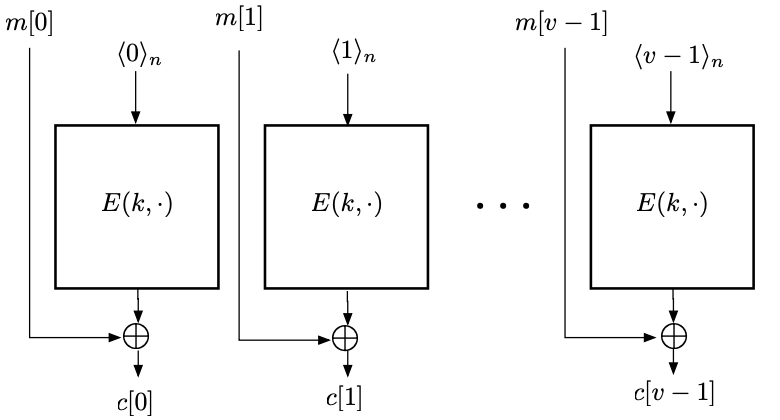
\includegraphics[width=0.65\linewidth]{figures/chapter4/fig13-a.png}}

  \subfigure[解密]{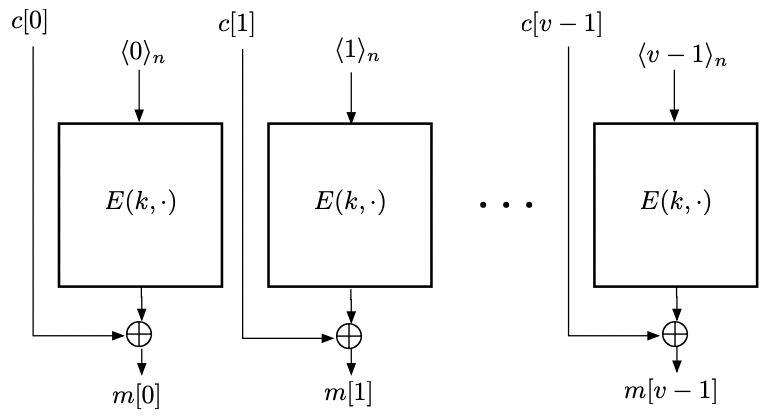
\includegraphics[width=0.65\linewidth]{figures/chapter4/fig13-b.png}}
  \caption{确定性计数器模式的加密和解密}
  \label{fig:4-13}
\end{figure}

\subsection{数学细节}

同之前一样,我们使用 \ref{sec:2-3} 中定义的术语对 PRF 给出一个更精确的数学定义。

\begin{definition}[伪随机函数]
一个\textbf{伪随机函数}包含一个算法 $F$,以及三个具有系统参数化 $P$ 的空间族:
\[
\mathbf{K}=\{\mathcal{K}_{\lambda,\Lambda}\}_{\lambda,\Lambda},\quad
\mathbf{X}=\{\mathcal{X}_{\lambda,\Lambda}\}_{\lambda,\Lambda},\quad
\mathbf{Y}=\{\mathcal{Y}_{\lambda,\Lambda}\}_{\lambda,\Lambda}
\]
它们满足:
\begin{enumerate}
	\item $\mathbf{K}$,$\mathbf{X}$ 和 $\mathbf{Y}$ 是可有效识别的。
	\item $\mathbf{K}$ 和 $\mathbf{Y}$ 是可有效采样的。
	\item 算法 $F$ 是一个确定性算法,对于输入 $\lambda\in\mathbb{Z}_{\geq1}$,$\Lambda\in{\rm Supp}(P(\lambda))$,$k\in\mathcal{K}_{\lambda,\Lambda}$ 和 $x\in\mathcal{X}_{\lambda,\Lambda}$,其运行时间以 $\lambda$ 的一个多项式为界,并且输出 $\mathcal{Y}_{\lambda,\Lambda}$ 中的一个元素。
\end{enumerate}
\end{definition}
和之前一样,在定义安全性时,攻击游戏是由安全参数和系统参数决定的,而优势是安全参数的一个函数。